\chapter{Wstęp}
\label{cha:Intro}
Wibrometria laserowa to technika pomiarowa pozwalająca na bezkontaktowe pomiary drgań powierzchni. Opiera się ona na odbiciu wiązki lasera, z którego można odczytać drgania powierzchni. Ponieważ pojedyncza wiązka lasera mierzy drgania pojedynczego punktu, problemem przy wykonywaniu takich pomiarów jest skanowanie drgań większych powierzchni. Dlatego też celem tej pracy jest konstrukcja systemu, który pozwoli na użycie wibrometru punktowego do przeskanowania powierzchni.

\section{Wibrometria laserowa \cite{Polytec_LDV}}
Wibrometr (\textbf{Laser Doppler Vibrometer}; \textbf{LDV}) to instrument służący do bezkontaktowych pomiarów drgań powierzchni. Wiązka lasera jest kierowana na mierzony obiekt, po czym wiązka odbita jest falą, o nieznacznie innej częstotliwości i fazie niż wiązka oryginalna. Zmiana ta jest proporcjonalna do drgań (ruchu) powierzchni, od której wiązka się odbiła.

\begin{figure}[h!]
\centering
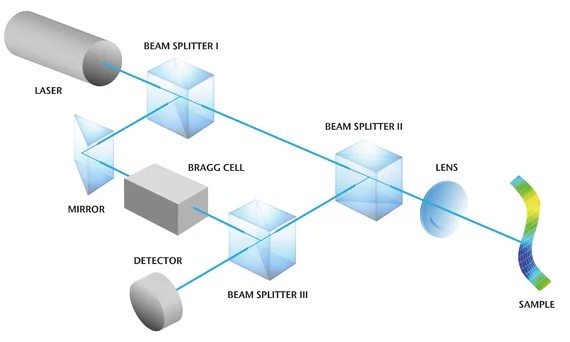
\includegraphics[width=0.8\textwidth]{img/ldv_inside.jpg}
\caption{Układ pomiarowy wewnątrz standardowego wibrometru laserowego. Źródło: \cite{Polytec_LDV}}
\label{img:ldv_inside}
\end{figure}

Wewnątrz wibrometru, rozdzielacz wiązki (Beam Splitter) rozdziela wiązkę laserową na wiązkę referencyjną oraz wiązkę pomiarową. Wiązka pomiarowa odbija się od mierzonego obiektu, po czym łączy się z wiązką referencyjną w operacji superpozycji i trafia na fotodetektor. (Przedstawione na rys. \ref{img:ldv_inside}.)

\subsection{Efekt Dopplera}
Podstawą działania wibrometru laserowego jest efekt Dopplera. Zgodnie z efektem Dopplera, zmiana częstotliwości wiązki pomiarowej względem wiązki odbitej jest proporcjonalna do szybkości ruchu obiektu oraz odwrotnie proporcjonalna do długości fali światła - zgodnie ze wzorem \ref{eq:doppler}. 

\begin{equation} \label{eq:doppler}
f_D = 2 \frac{v}{\lambda}
\end{equation}

Wzór \ref{eq:doppler} pozwala na wyznaczenie prędkości mierzonego obiektu na podstawie zmiany częstotliwości wiązki światła. Natomiast sama zmiana częstotliwości jest wyznaczana z superpozycji wiązek za pomocą interferometrii.

\subsection{Interferometria}
Wspomniano powyżej, że na fotodetektor trafia superpozycja wiązki referencyjnej oraz odbitej. Interferometria to technika stosująca interferencję fal w superpozycji do ekstrakcji informacji z tych fal, wykorzystywana właśnie w tym celu w wibrometrze. \cite{history_of_science_and_tech}

Przykładowo, jeżeli obie fale mają tą samą częstotliwość, interferencja dwóch fal pozwala na łatwe wyciągnięcie informacji o przesunięciu w fazie między tymi dwoma falami. Jeżeli fale zupełnie się wygasiły, oznacza to, że strzałka naszła się z węzłem i przesunięcie w fazie wynosi dokładnie pół długości fali.Jeżeli strzałki się wzmocniły, oznacza to, że nie ma przesunięcia w fazie. Natomiast w każdym innym wypadku można łatwo obliczyć przesunięcie na podstawie pozycji węzłów i strzałek nowej fali. \cite{Two_laser_interferometry}

W przypadku wibrometrów laserowych, mierzona jest interferencja intensywności światła wiązek, zgodnie ze wzorem \ref{eq:l_interference}. \cite{Polytec_LDV}

\begin{equation} \label{eq:l_interference}
I_{tot} = I_1 + I_2 + 2 \sqrt{I_1 I_2} \cos{ \frac{2 \pi (r_1 - r_2)}{\lambda}}
\end{equation}


\subsection{Typy wibrometrii laserowej \cite{Polytec_LDV_typology}}
\begin{itemize}
    \item \textbf{Punktowa} - najprostszy sposób pomiaru, pojedyncza wiązka mierzy drgania pojedynczego punktu.
    \item \textbf{Różnicowa} - pomiar drgań w dwóch punktach, które wibrują relatywnie do siebie nawzajem.
    \item \textbf{Skanująca} - wiązki lasera skanują badany przedmiot tworząc mapę punktów.
    \item \textbf{Rotacyjna} - pomiar faktycznej prędkości rotacyjnej przedmiotów.
    \item \textbf{Mikroskopowa} - pomiar drgań małych obiektów.
    \item \textbf{Płaszczyzny} - pomiar drgań i ruchu płaszczyzn poruszających się prostopadle do wiązki lasera.
    \item \textbf{Wielopunktowa} - pomiar macierzą wiązek lasera.
\end{itemize}


\section{Wibrometria skanująca}
\subsection{Powszechnie stosowane rozwiązania w wibrometrii skanującej}
\label{cha:polytec_scan}
Najbardziej powszechnym rozwiązaniem pozwalającym na przeskanowanie powierzchni są trzy głowice z zamieszczonymi lustrami. Wspomniane głowice są stacjonarne. Jedynie lustra, odbijające wiązkę lasera w wybranym kierunku, są ruchome - obracają się dookoła osi z. Jest to rozwiązanie opierające się na dobrym rozłożeniu głowic, tak aby ruch wiązki wzdłuż zaledwie jednej osi dał pełen obraz skanowanego przedmiotu. Przykładem takiego systemu jest np. PSV-500-3D, przedstawiony na zdj. \ref{img:ldv_3d}. \cite{Polytec_LDV_3D}

\begin{figure}[h!] 
\centering 
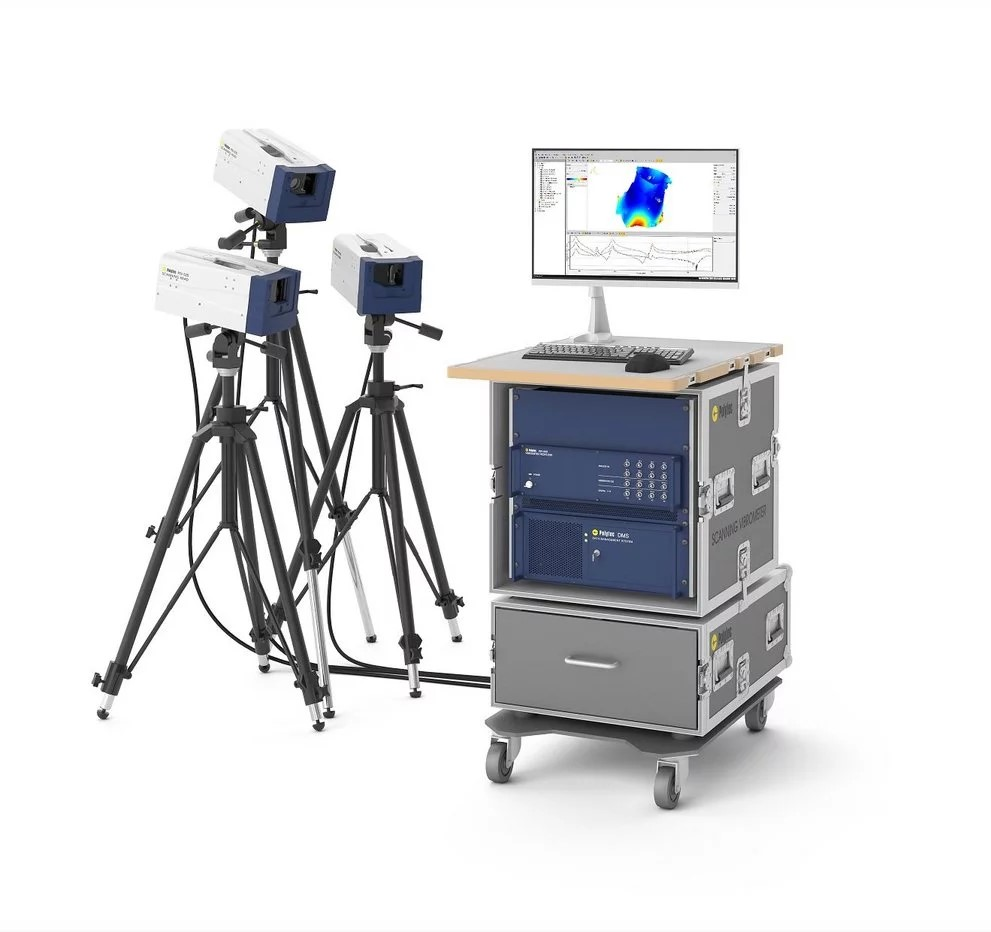
\includegraphics[width=0.6\textwidth]{img/ldv_3D.jpg}
\caption{System PSV-500-3D. Źródło: \cite{Polytec_LDV_3D}}
\label{img:ldv_3d}
\end{figure}

\subsection{Rozwiązanie zaproponowane w tej pracy}
Podstawowym problemem wibrometrii skanującej jest cena rozwiązania przedstawionego w \ref{cha:polytec_scan}. Cena zestawu trzech głowic skanujących jest bardzo wysoka.

Celem pracy jest skonstruowanie systemu, który pozwoliłby przeskanować powierzchnię, używając pojedynczej głowicy wibrometru punktowego. Można to osiągnąć na kilka różnych sposobów. Dwa rozważane na potrzeby tej pracy to:

\textbf{Ruchome lusterko} - Umieszczenie ruchomego lusterka przed wibrometrem, tak aby wiązka laserowa odbiła się od niego.

\textbf{Ruchomy wibrometr} - Umieszczenie całej głowicy wibrometru na stole, obracającym się dookoła osi $z$ oraz $y$, co pozwala celować całym wibrometrem w wybrany punkt na sferze dookoła wibrometru.

 W rozwiązaniu z obracającym się lusterkiem należałoby wziąć poprawkę na odbicie wiązki od lusterka. Odbicie takie wprowadza załamanie się wiązki i co za tym idzie, zmianę trasy wiązki laserowej. Wprowadza to wymóg przeprowadzanie skomplikowanych obliczeń na sygnale wyjściowym wibrometru. Rozwiązanie z lusterkiem wprowadziłoby także strefę martwą centralnie przed wibrometrem. Uniemożliwiłoby to pomiar punktów znajdujących się w tej strefie. Wymusiłoby natomiast pomiar punktów znajdujących się pod odpowiednim kątem do osi wibrometru.
 
 Ostatecznie zdecydowano się na wersję drugą, ruch całym wibrometrem. Jest to rozwiązanie koncepcyjnie prostsze ale wymaga mocniejszych silników i większego systemu pozycjonującego, co wprowadza inne wyzwania.